\section{引言}

\subsection{研究概述}

\subsubsection{研究背景}
1950年,艾伦·图灵提出图灵测试\cite{XSYK202306001},成为评估机器智能水平的重要参照。六年后,“人工智能”一词在美国达特茅斯会议中正式确立,标志着新研究领域的开启。人工智能随时代演进,至今已发展成为一门跨越计算机科学、信息科学、心理学、哲学、认知神经科学及生理学等多个学科的尖端交叉学科 \cite{YUAN200905001},尤其体现在大规模预训练语言模型(又名“基座模型”或“大模型”)的崛起,此类模型凭借庞大的参数规模构建起复杂的神经网络结构\cite{bommasani2022opportunities}。这一技术创新与应用具有里程碑意义,引领研究者跨入通用人工智能研究的新纪元 \cite{ZXTX20240416002}。

\begin{figure}[ht]
  \centering
  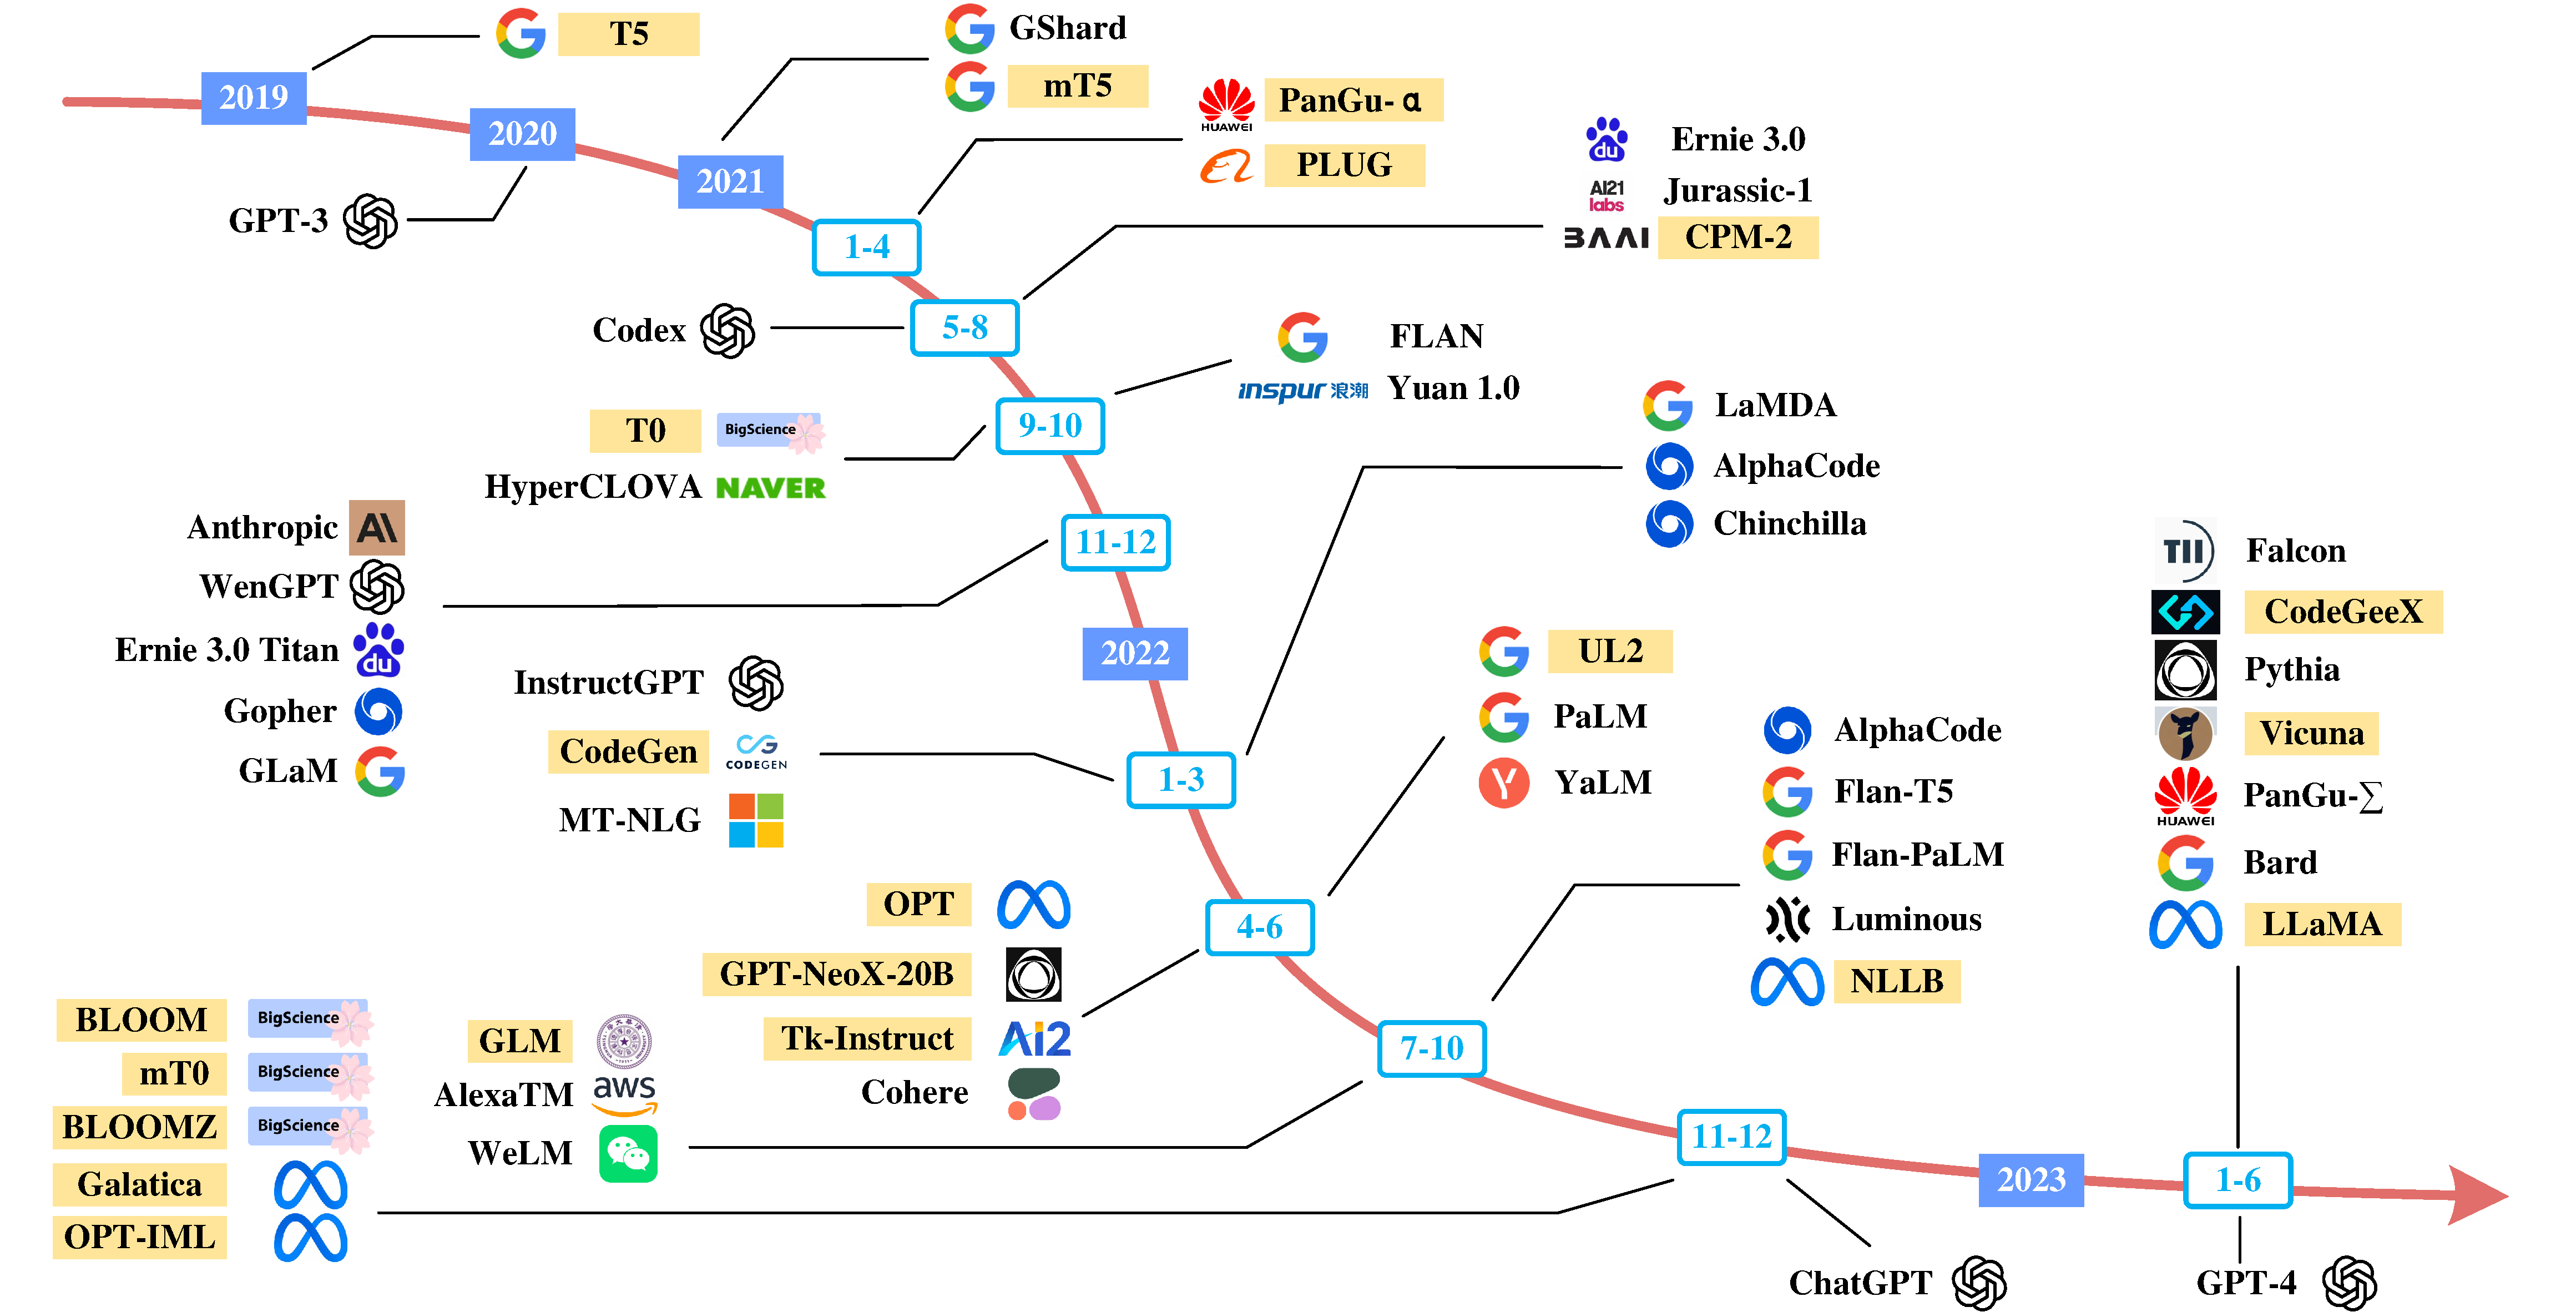
\includegraphics[width=1.0\textwidth]{./Img/大模型发展绘图.pdf}
  \caption{国内外大语言模型整体发展示意}\label{fig:a-00}
\end{figure}

国内外的大模型发展如图 \ref{fig:a-00} 所示,在2020年,OpenAI首次提出的“规模定律”揭示了模型性能随参数规模、数据量及训练持续时间呈指数增长而接近线性提升的趋势,此举显著降低了对传统架构优化及超参数调优的依赖。自此之后,学术与工业界的关注点集中于开发大规模语言模型,其中 GPT-3 \cite{brown2020language} 作为首个达到千亿参数级别的模型,在自然语言处理(NLP)领域实现了多项任务的革新,彰显出前所未有的零样本与少量样本学习效能,为巨型预训练模型时代拉开了序幕。

这一进展进一步激发了科技巨头如谷歌、Meta的竞争,纷纷推出百亿乃至千亿参数量级的模型,例如Gopher、Chinchilla、PALM等,这些模型的参数量达到了数十亿甚至数千亿。在2022年,大模型展现出的卓越性能在全球范围内引发了研发热潮,众多大模型如雨后春笋般涌现,国际上InstructGPT、MT-NLG、OPT、LLaMA-2、Flan、Luminous和ChatGPT \cite{chatgpt2022} 等大模型相继发布。与此同时,国内也推出了GLM-130B、ChatGLM2、WeLM、PanGu等重要的大模型。这些模型的发布进一步丰富了大模型生态系统,使其显得更加充满活力。

\begin{figure}[h]
  \centering
  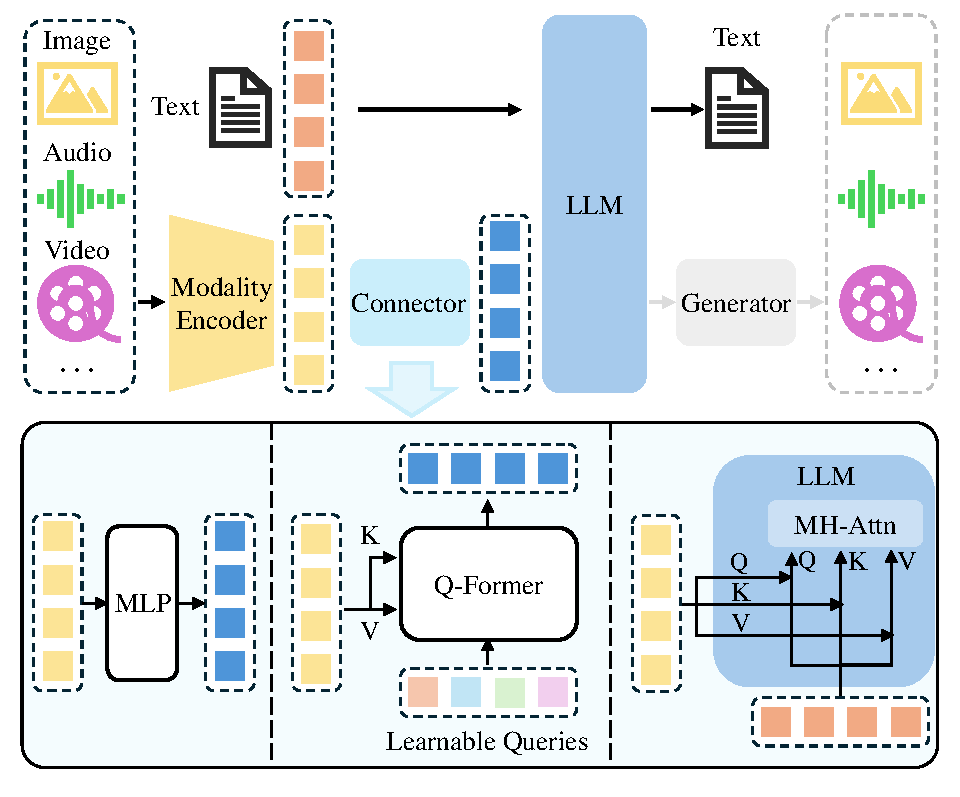
\includegraphics[width=0.8\textwidth]{./Img/多模态大模型结构.pdf}
  \caption{多模态大模型结构}\label{fig:a-01}
\end{figure}


\begin{figure}[ht]
  \centering
  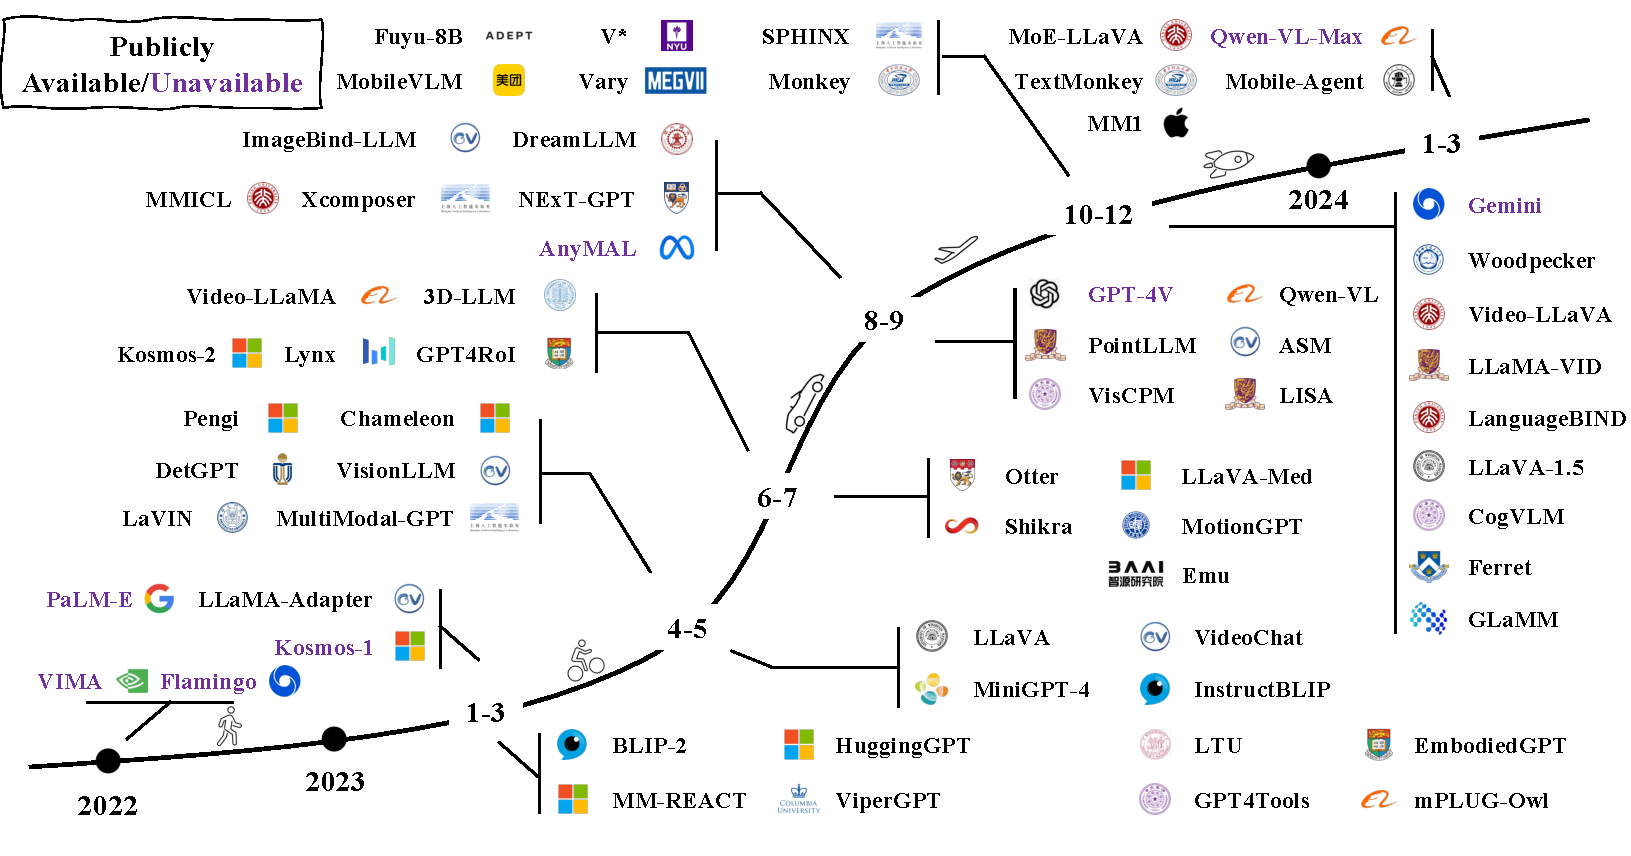
\includegraphics[width=1.0\textwidth]{./Img/多模态大语言模型.pdf}
  \caption{国内外多模态大语言模型发展示意}\label{fig:a-02}
\end{figure}


在图 \ref{fig:a-00} 展示的大语言模型宏观格局中,一个突出的现象是大多数模型集中在单一模态任务上,即文本到文本的生成。然而,自2022年以来,一种新型的多模态大语言模型(MLLM)开始崭露头角,它们能够跨越文本、图像和视频这三种不同模态的界限,实现不同模态间的自由生成。这些多模态大型模型的普遍的内部结构如图 \ref{fig:a-01} 所示\cite{yin2024survey},它包括一个编码器(Encoder)、一个连接器(Connector)和一个大语言模型(LLM)。 大语言模型可以附加一个可选的生成器,以生成除文本之外的更多模式。 编码器接收图像、音频或视频并输出特征,这些特征由连接器处理,以便大语言模型可以更好地理解。 其中连接器大致分为三种类型:基于投影的连接器、基于查询的连接器和基于融合的连接器。 前两种类型采用令牌级融合,将特征处理成令牌与文本令牌一起发送,而最后一种类型则在大语言模型内部实现特征级融合。

在这类框架的基础上,多模态大语言模型引发了一场前所未有的研发热潮,在图 \ref{fig:a-02} 中,我们可以看到多模态大语言模型(MLLM)的发展历程。黑色和蓝色的线条分别代表开源和闭源模型,清晰地展示了它们在时间轴上的进展。2022年标志着多模态大语言模型的诞生,其中 VIMA 和 Flamingo 作为该领域的先驱模型,为后续的发展奠定了基础。然而,对于多模态大语言模型(MLLM)而言,真正的转折点出现在2023年,在这一年,我们目睹了一场前所未有的技术革新浪潮,多模态大语言模型的发展呈现出爆炸性的增长。全球科技巨头们在这一年里竞相推出了他们的创新模型,如谷歌(Google)、Meta、微软(Microsoft)、阿里巴巴(Alibaba)、OpenAI,以及苹果(Apple)等领先科技公司纷纷展示了他们在MLLM领域的最新研究成果。

除了工业界之外,学术界同样展现出了强劲的竞争力和创新精神。2023年,不仅是科技公司的丰收年,也是学术界的重要里程碑。新加坡国立大学、南洋理工大学、清华大学、北京大学、香港大学、复旦大学以及上海交通大学等全球顶尖高等学府的师生们在这一年中,通过他们的智慧和努力,为多模态语言理解技术的理论和应用实践做出了显著贡献。这些学府的研究成果,无论是在深化理论研究,还是在推动技术应用方面,都极大地拓展了MLLM的边界。他们的工作不仅加速了学术交流,也为工业界提供了宝贵的知识和技术支持,促进了整个领域的健康发展。图 \ref{fig:a-02} 以其详尽的时间线和关键的模型发展节点,绘制出了2023年多模态大语言模型的蓬勃发展图景。这一年,MLLM的发展达到了一个新的高潮,成为了全球科技竞争和合作的一个缩影。它不仅标志着多模态语言理解技术的一个关键转折点,更预示着人工智能技术未来发展的方向和趋势。

随着人工智能技术的突飞猛进,尤其是多模态大型语言模型(MLLM)的应用,我们在处理复杂任务方面的能力得到了显著提升。这些模型通过先进的文本生成技术,即自然语言处理(NLP)的核心,不断推动着智能系统的边界。在这样的技术浪潮推动下,我们本次的研究专注于探讨人工智能大背景下的两个领域出发:

\begin{itemize}[leftmargin=3em]
    \item \textbf{大数据技术}:驱动气象预测的精准化转型与效能优化。
    \item \textbf{人工智能技术}:基于计算机视觉图像检索图像的的深化研究与应用实践。
\end{itemize}

通过人工智能与数据科学的紧密融合,为气象预测及大规模细粒度图像检索领域带来了前所未有的革新动力与广阔前景,显著增强了这些领域的预测精度与检索效率。

\subsubsection{研究意义}

在大模型技术的强力驱动下,研究领域迅速拓展,深入涉及深度学习、机器学习、智慧教育、个性化学习、自适应学习、情感计算、学习分析以及教育大数据等多个尖端且关键的主题领域。鉴于此,本研究计划专注于人工智能在气象预测优化及大规模图像处理的双重应用领域,旨在通过深化AI技术的研究与创新实践,提升气象预测的精确性以及模型的鲁棒性,并优化资源调度的效率。同时,针对大规模图像数据处理中对于高精度识别与分析的迫切需求,尤其是在细粒度图像检索、人脸识别、目标检测及语义分割等关键技术环节,我们将积极探究并推广人工智能算法的高效应用途径,进一步拓宽人工智能技术在气象预测分析及大规模图像智能处理领域的应用边界与发展潜力。

\textbf{气象预测}是气象学、应急管理和多个依赖气候条件行业的核心关注点,它运用统计学、机器学习、人工智能等技术手段,旨在预测特定地区未来一段时间内的天气状况,包括温度、降水、风力等关键指标,对农业规划、能源分配、交通运输及公众安全等领域具有重要指导意义。在气象预测领域 \cite{HJKZ2024011600J},我们融合了大数据与深度学习的最新研究成果,运用历史气象数据挖掘气候模式,旨在揭示天气变化的内在规律,并实现对气象变量多维度的精密解析。通过融合时间序列分析、灵活的机器学习模型及深层神经网络,我们能够快速适应天气系统变化,实时监控气象,准确预测极端事件,优化调度策略,为气象服务、灾害预警及保障公共安全提供智能辅助决策,提升气象预测的准确率与应变效率。

\textbf{大规模细粒度图像检索}(Large-scale Fine-grained Image Retrieval)是一种专注于在庞大图像数据库中,精准查找具有细微差异的同类物品图像的技术。与一般的图像检索不同,细粒度检索关注的是那些属于同一类别但存在微小差异的对象,比如不同种类的鸟类、植物、汽车型号或服装款式等。在图像检索领域,深度学习和多模态大模型的发展,极大地提升了图像识别和分类的准确性。这些技术在处理大规模图像数据集时,能够通过学习细粒度特征,实现高效、精确的图像匹配和检索。例如,通过结合卷积神经网络(CNN)\cite{LeCun2015}和Transformer \cite{vaswani2023attention} 的架构,可以对图像进行深度分析,提炼出高度抽象且富有代表性的特征,提高检索的准确性和泛化能力。

\subsection{研究现状与方法}

\subsubsection{研究现状}

在\textbf{气象预测}这一研究领域,马飞等(2024)\cite{JYGC20240415002} 提出一种融合气象和交通特征数据的GAF-CNN-LSTM短时交通流预测方法,通过将时间序列数据转换为图像并利用深度学习提取特征,显著提升了预测精度。沈金星等(2024)\cite{HJKZ2024011600J} 结合了CNN、LSTM以及注意力机制三个模块,有效捕捉了气象特征的时序非线性变化,显著优于对比模型。马国斌等(2011)\cite{ZHXU201103002} 基于自然灾害风险理论,利用GIS空间分析功能和归一化及层次分析法,对中国进行了洪涝灾害危险性评估,开发了一个全国洪涝灾害危险性评估模型,并以此为基础生成预警产品,为防灾减灾提供决策支持。陈聪等(2023)\cite{1023751652ch} 针对暴雨灾害,提出了集成经验模态分解-马尔科夫(D-Markov)模型;同时针对大气污染问题,设计了基于卷积门控循环单元(CNN-GRU)的预测系统。通过实验验证,这两种模型都能提供高精度的预测结果,为防灾减灾提供了有力支持。屈峰等(2024)\cite{HBYD202401011} 提出一种结合小波分析、LSTM网络和卡尔曼滤波技术的混合方法,有效预测短期风速变化趋势,并通过实证分析验证了其预测性能。申洪涛等(2024)\cite{DLJS202401002} 提出一种结合小波分析、LSTM网络和卡尔曼滤波技术的混合方法,有效预测短期风速变化趋势,并通过实证分析验证了其预测性能。Charlton-Perez 等(2024)\cite{charltonperez2024ai} 通过分析机器学习模型对高影响天气事件——风暴Ciarán的预测表现,揭示了这些模型在模拟宏观天气结构方面的准确性,但在细节捕捉上存在局限,指出了机器学习在天气预测精度提升上需要进一步研究的必要性。


\textbf{细粒度图像检索}源自于人工智能领域中细粒度图像分析方面\cite{wei2021finegrained}的一个基本主题,近年越来越受到重视\cite{solving9157668}\cite{cui2020exchnet}\cite{zheng2019towards}。依据查询图像的本质特性,细粒度图像检索任务可被区分为两大类别:一是基于内容的细粒度图像检索(FG-CBIR),二是基于草图的细粒度图像检索(FG-SBIR)。具体地,早期在FG-CBIR领域中,研究工作如 SCDA \cite{wei2017selective} 引入了深度预训练网络的应用,而这一过程并不依赖于明确的局部化监督信息。随后,为了解决无监督检索在准确率上的局限性,一系列基于监督的度量学习策略应运而生 \cite{HoIH8237325},旨在通过引入额外的指导信号来优化检索性能。

在另一研究轨迹上,基于手绘草图的图像检索(FG-SBIR)作为一个引人注目的领域,专注于将手绘草图作为查询工具,以便精确地从现实照片中找到对应物体。这一领域是细粒度图像检索与跨模态检索交汇的核心。现有技术,如文献\cite{Yu7780462SMTS}\cite{song8237854DSA}所展示,关键在于构建一个嵌入空间,使得草图和照片可以在此空间中通过最近邻搜索高效匹配。尽管当前的细粒度图像检索方法通常依赖深度网络的最终特征层输出来进行检索,并在一些场合取得了显著效果,但面对大规模数据集时,这些方法的局限性显而易见。特别是在大规模图像检索任务中,要实时找到与查询最匹配的精确最近邻,常常面临巨大的时间成本挑战,有时在实际执行中几乎不可行。

面对这一挑战,细粒度哈希技术应时而生,被视为一个极具潜力的解决方案。该技术旨在生成紧凑的二进制编码,以高效地捕捉和表征细粒度对象的独有属性,因此近年来在细粒度图像检索的研究界获得了广泛关注 \cite{solving9157668}\cite{Zeng_2024}\cite{DSH9037360}。

\subsubsection{研究方法}

\textbf{数据处理的创新}:
在气象预测研究中,我们采用前向填充策略处理缺失值,即用时间序列的均值填补,同时排除了缺失三个及以上指标的记录以保证数据质量。所有数据在模型训练前都经过归一化,以统一数据范围,优化模型学习效率和预测准确性。在图像检索研究中,鉴于图像尺寸参差不齐,我们针对每一张图像放大为 $256 \times 256$,然后针对训练图像和测试图像分别采用随机裁剪为$224 \times 224$和中心裁剪为 $224 \times 224$ 两种方式,最后按照国际公认的标准进行归一化,最后得到标准的RGB三通道的图像数据,确保评估模型时所使用图像数据的公平性。

\textbf{气象预测技术的创新}:在气象预测领域,长短期记忆网络(LSTM)因其在处理时间序列数据方面的独特优势而备受青睐。LSTM网络通过其精巧的门控机制,能够有效捕捉时间序列中的长期依赖关系,这对于模拟气象现象中复杂的动态变化至关重要。鉴于气象变化的精细时间关联和不可预测性,LSTM在揭示气象数据内在规律方面展现出了卓越的能力。此外,LSTM模型与卷积神经网络(CNN)、小波分析以及多种优化算法的结合使用\cite{HJKZ2024011600J}\cite{JYGC20240415002}\cite{HBYD202401011}\cite{DLJS202401002},进一步扩展了其在气象预测研究中的应用潜力。受混合网络模型的启发,我们设计了一个结合了卷积神经网络(CNN)和长短时记忆网络(LSTM)互补优势的混合模型。在模型训练阶段,我们通过特征工程精心筛选了对预测任务至关重要的特征,并通过对学习率、批量大小和迭代次数等超参数的精细调整,优化了模型的性能。在评估过程中,我们采用了均方误差(MSE)和平均绝对百分比误差(MAPE)等指标来量化模型的预测效能,以确保我们的混合模型能够在气象预测任务中提供高精度的预测结果。

\textbf{图像检索技术的创新}:在图像检索的研究领域,我们提出了一种创新的细粒度哈希检索框架,命名为LGESD(Local and Global learning of Explicit Spatial Decay)。该框架的设计精髓在于其独特的双层结构,这一结构融合了全局哈希映射单元与局部哈希映射单元,旨在生成能够同时捕获图像全局语义信息和局部细节信息的二进制哈希码。这种设计显著提升了哈希码的表达能力和图像检索任务中的区分度。同时,在注意力机制的改进上,LGESD框架创新性的设计了显式空间衰减注意机制(ESD),这一机制在生成全局和局部特征时,通过考虑特征之间的空间关联性和衰减特性,确保了特征的互补性并增强了特征的唯一性。这种显式建模特征间的空间关系的方法,为图像检索任务提供了更为丰富和鲁棒的特征表示。在一系列实验中,我们展示了LGESD框架在多个标准图像数据集上的性能,验证了其在图像检索任务中的准确性和泛化能力。实验结果表明,LGESD框架在处理细粒度图像检索任务时,相较于现有技术,展现出了显著的性能优势。

